%=======================+=========================
%================  Reconstruction  ================
%=================================================


\section[Event reconstruction]{Event reconstruction \label{sec:reconstruction}} 

% Copy from GlueX-doc-3108
% "Production and Analysis of GlueX Data"
% TODO: UPDATE for 2017

\GX~uses the computer center batch farm at JLab to perform data monitoring, event reconstruction, and physics analyses.  For data monitoring, detector hit occupancies, calibration and reconstruction quality, and experimental yields and resolutions, are analyzed for several physics channels.  A subset of the data is monitored automatically as it is saved to tape.  Every few weeks, monitoring processes are launched on a subset of the data to study improvements from ongoing calibrations and reconstruction software improvements.  The histograms produced by these monitoring jobs are displayed on a website and ROOT files are available for download, enabling the collaborators to easily study the quality of the data. 

Every few months, a major reconstruction launch over all of the data is performed, linking hits in the various detector systems to reconstruct particles in physics events.  Monitoring plots from these launches are also published to the web. Finally, regular analysis launches over the reconstructed data are performed, where a JANA plugin filters out reactions previously specified by users in a web form. The results of these launches are saved in reaction-specific ROOT TTrees for further analysis.

For all launches, JANA is run in a multi-threaded mode to make efficient use of the available computing resources. Fig.\,\ref{fig:offline_monitorA} shows the multithreaded scaling from our monitoring launches. The program performs near the theoretical limit for jobs that use a number of threads that is less or equal the number of physical cores on the processor. By using hyperthreads, a smaller but still significant gain is achieved.
%SWIF is used to manage the batch farm jobs, and is queried to study the performance of the launches.  Figure~\ref{fig:farm-time} shows how many batch farm jobs were in each processing state as function of time our latest reconstruction launch.
All file outputs are written to a write-through cache system, which is ultimately backed up on tape.

\begin{figure}[h!]\centering
%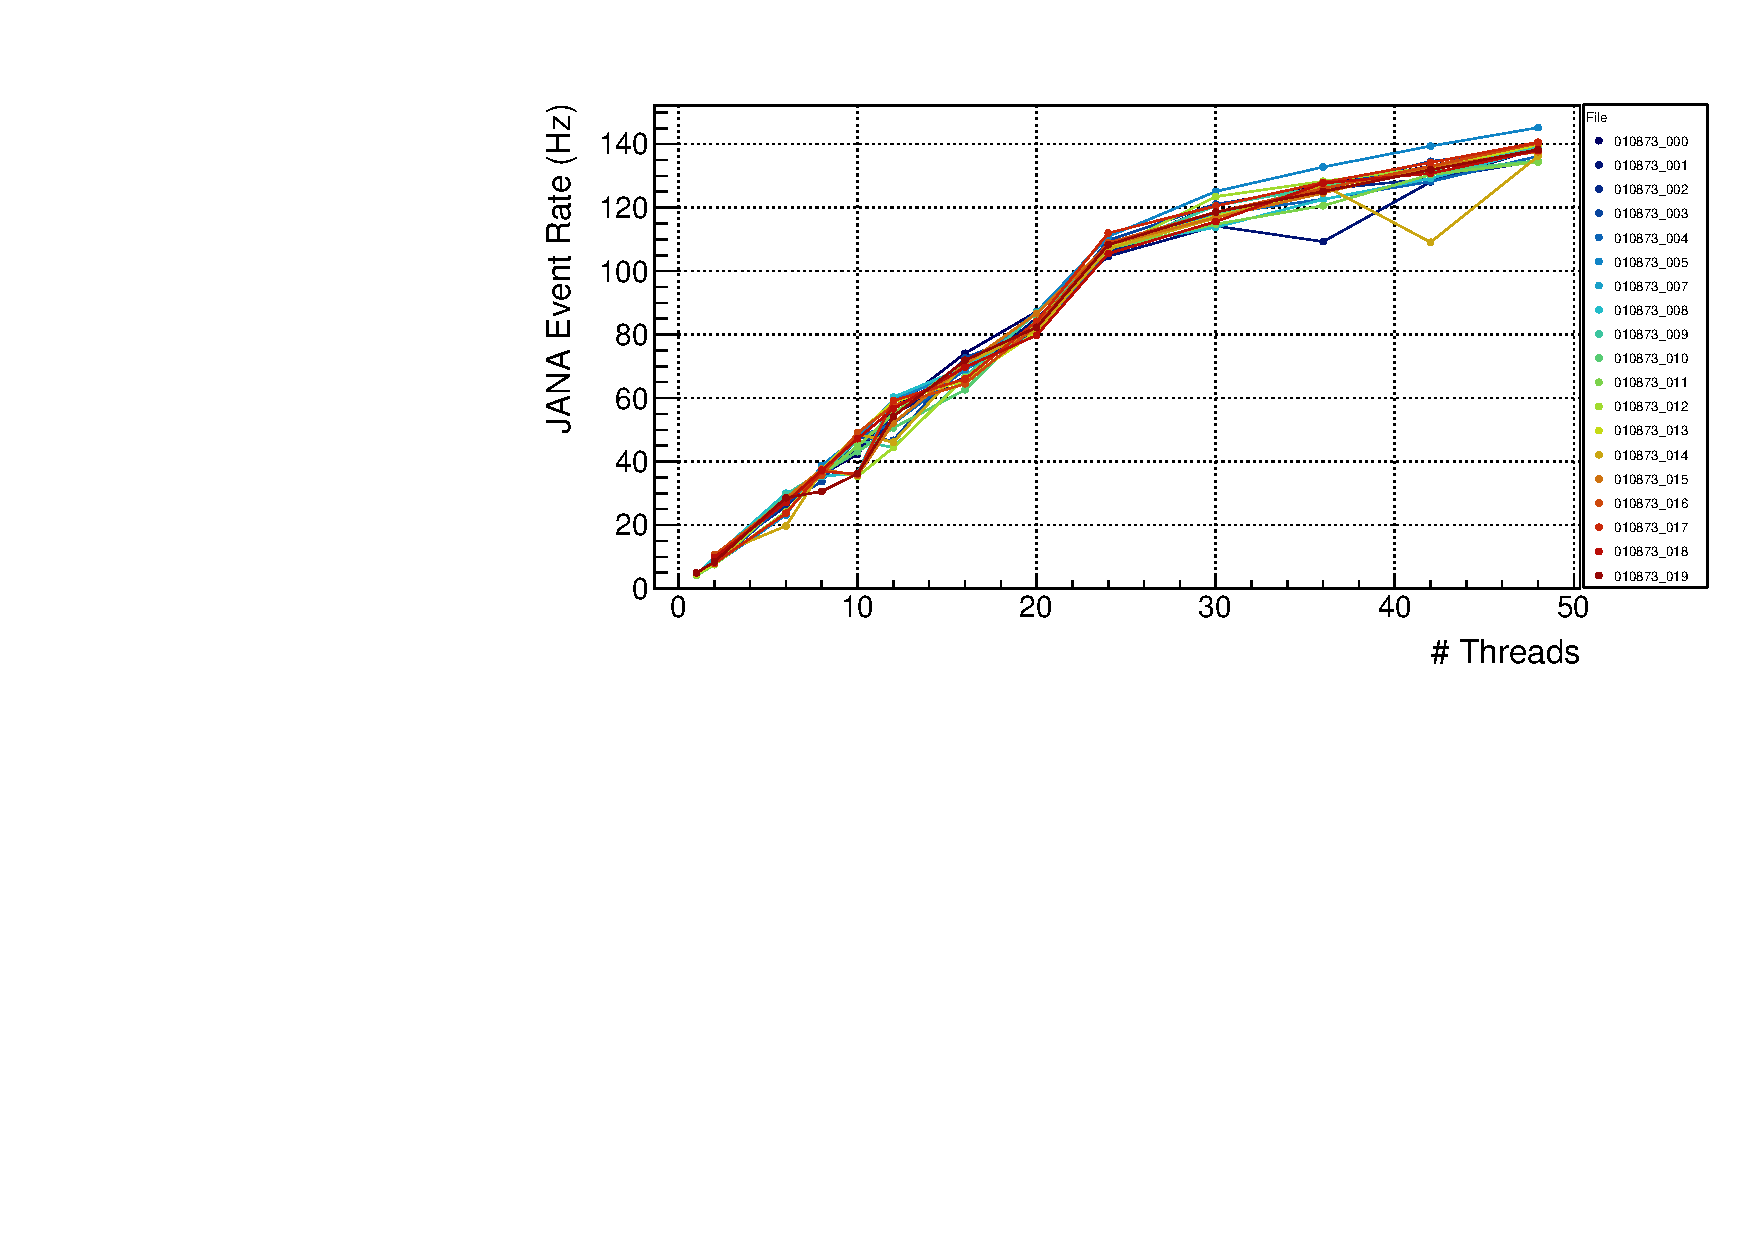
\includegraphics[width=0.7\textwidth]{figures/OfflineMonitor_PlotA.pdf}
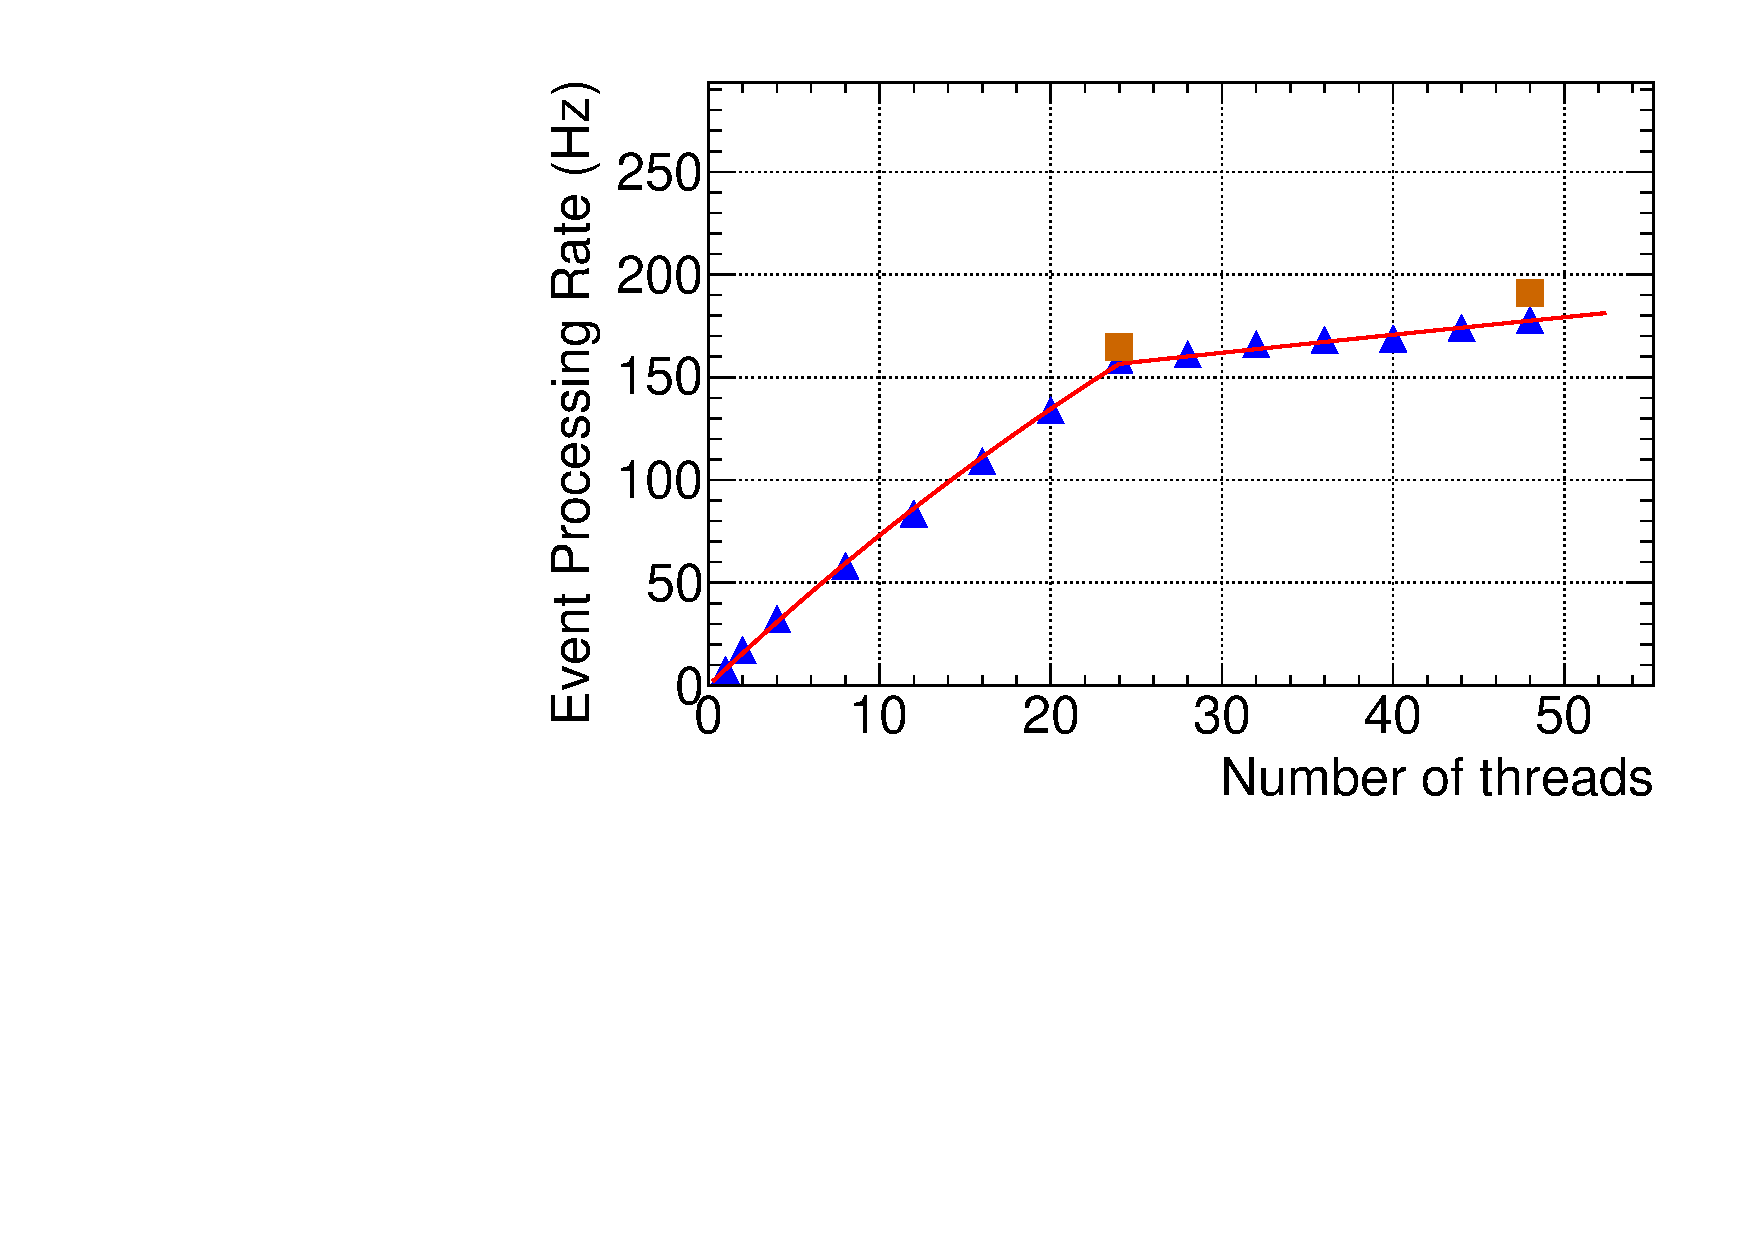
\includegraphics[width=1.0\textwidth]{figures/rate_vs_nthread.pdf}
\caption[]{\label{fig:offline_monitorA}The scaling of program performance as a function of the number of processing threads. The computer used for this test consisted of 24 full cores (Intel x86\_64) plus 24 hyperthreads. The orange squares are from running multiple processes, each with 12 threads.} 
\end{figure}

\GX~has recorded about 1400 separate physics-quality runs, with a total data footprint of about 3 petabytes. Data were saved in 19-GB files, with all runs consisting of multiple files (typically $100$ or more per run). Fig.\,\ref{fig:production_overview} shows an overview of the different production steps for \GX~data, which are described in more detail in the following subsections.

\begin{figure}[hbt]\centering
%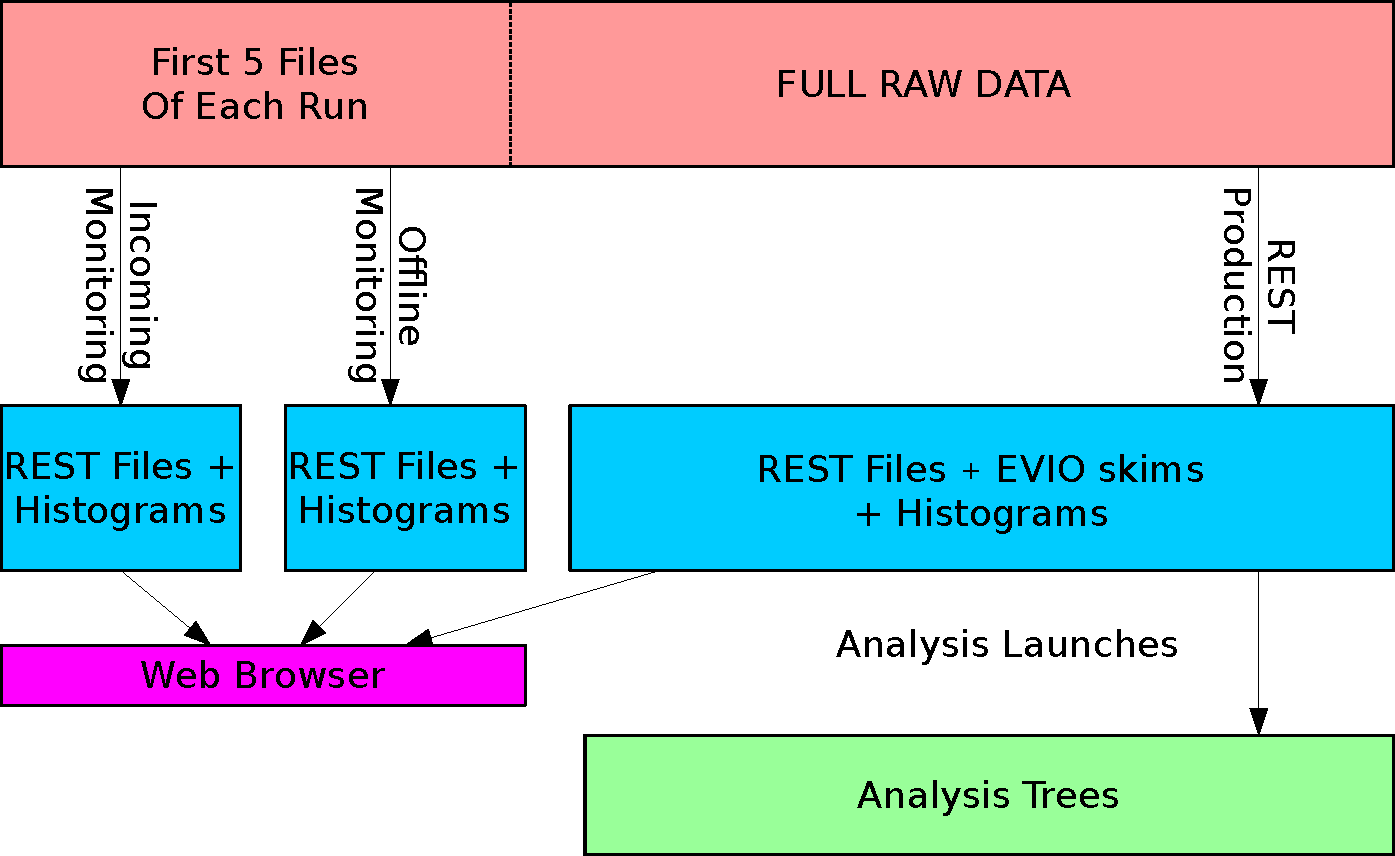
\includegraphics[width=0.8\textwidth]{figures/Production_generic.pdf}
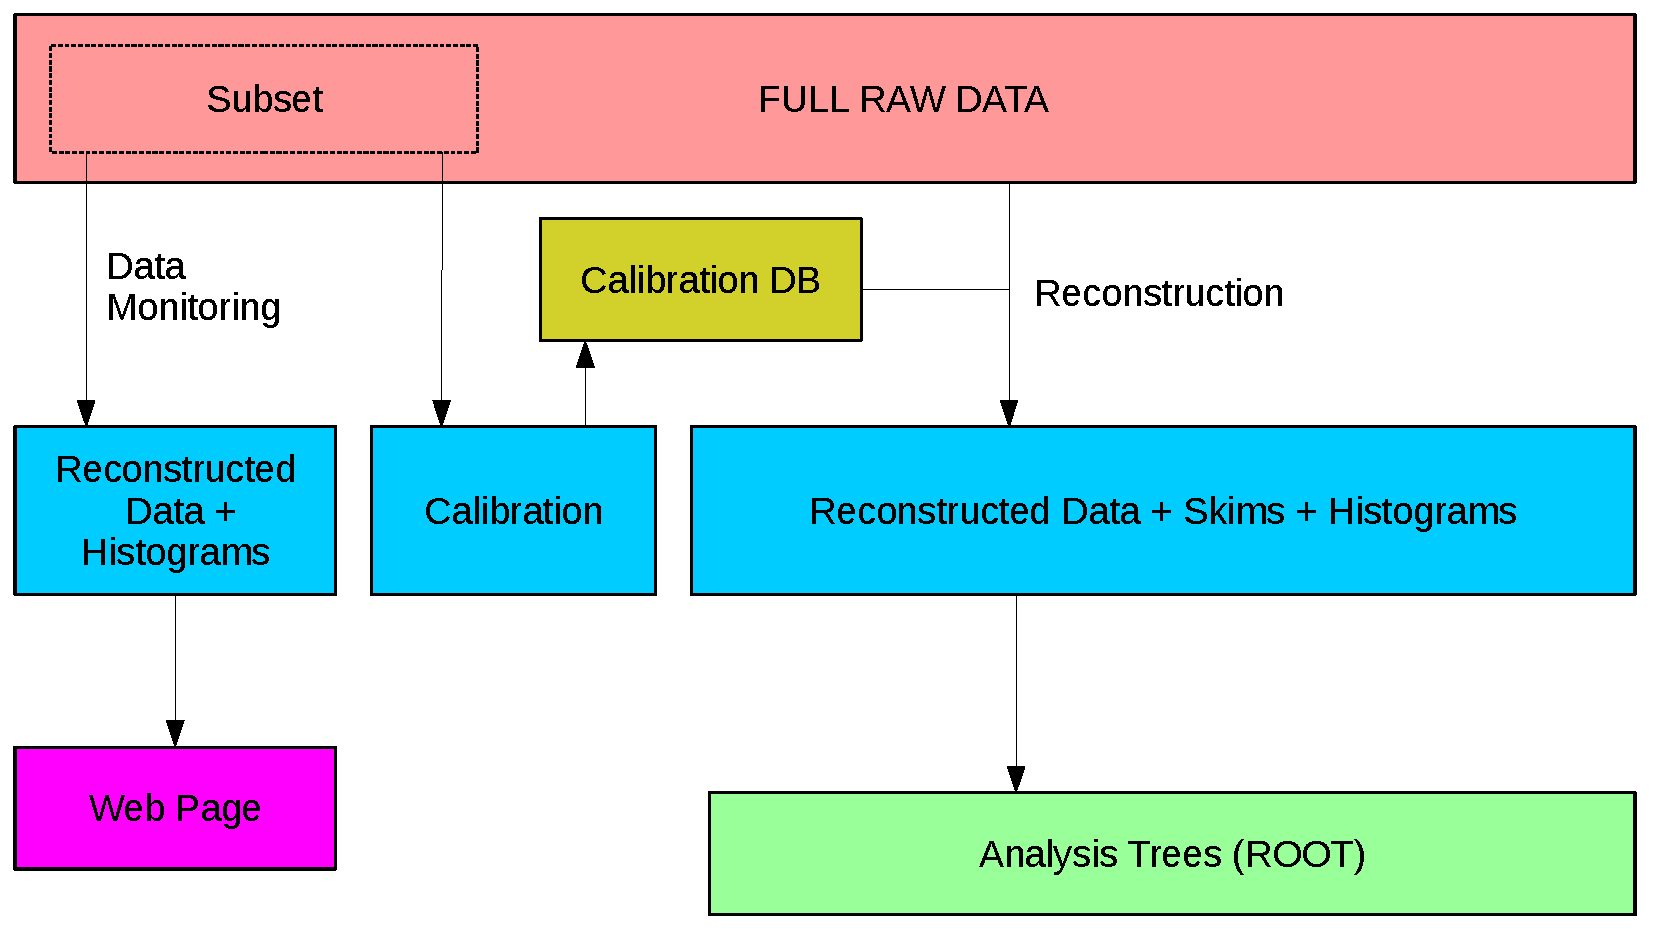
\includegraphics[width=0.9\textwidth]{figures/production_overview_calib_v2.pdf}
\caption[]{\label{fig:production_overview}Production flowchart for \GX~data, illustrating analysis steps.} 
\end{figure}

%--------------------------------------------------------------------------
\subsection{Calibration \label{sec:reccalibration}}

Two types of calibration jobs are run, depending on the complexity of the calibration procedures.  Simple, well-understood calibrations such as timing alignment between individual channels and subdetectors or drift chamber gain and time-to-distance calibrations, can be performed with one file of data per run.  These procedures are run either in the online environment or on the batch farm, and can be run several times as needed following any improvements in reconstruction algorithms or other calibrations.

More complicated calibration procedures, such as calorimeter gain calibration, require more data and are often iterative procedures, requiring several passes through the data.  The raw data is processed upon arrival on the batch farm, resulting in histograms or in selected event data files in EVIO or ROOT tree format.  Many of these outputs require that charged particle tracks be reconstructed, but because of the computationally intensive nature of track reconstruction in \GX, the available computing resources at JLab are insufficient to fully reconstruct all the raw data as it comes in.  Therefore, only about $10-20$\% of the data has the full suite of calibration procedures applied.  Processing of the remaining data is mostly focused on separating out, or ``skimming,'' events collected by specialized triggers. 
The individuals responsible for specific detector calibrations are then responsible for analyzing the skimmed data.

%--------------------------------------------------------------------------
\subsection{Monitoring \label{sec:recmonitoring}}

The red-colored box at the top of Fig.~\ref{fig:production_overview} represents experimental data that has been copied to the computer center and backed up to tape. The left-hand section of the box labeled ``subset" represents the first five files of each run, which are run through offline monitoring processes. These monitoring jobs are first processed during the run to check the quality of the data, but are also processed after major changes to calibrations or software to validate those changes. These jobs produce Reconstructed Events Storage (REST) files and ROOT histogram files for checking the detector and reconstruction performance.

%--------------------------------------------------------------------------
\subsection{Reconstruction \label{sec:recreconstruction}}

When the data is sufficiently well calibrated, a full production pass on the physics quality data is performed. In the current total \GX~data set, about 1400 runs were deemed ``physics quality." The remaining runs were short runs related to engineering and commissioning tests of the experiment; while this remainder is small compared to the total number of runs, it includes the vast majority of all data recorded during the running period, representing about 3 petabytes. All these files were reconstructed using computing resources at several sites, equivalent to more than 20 million core-hours combined. This produced more than $500$ terabytes of REST data files. The large reduction in size from collected event data to physics data files (about a factor of six) permits faster and more efficient physics analyses on the data.
%, and is also small enough to be fully exported to off-site computer centers, see section~\ref{sec:remote-dist} (not really).

During the REST production, a series of detector studies were performed that required access to raw data and that would not be possible on the reconstructed data alone. Many improvements to software and detector calibration resulted from these studies. Similar studies can be made with simulated data to match and assess the detector acceptance.

%--------------------------------------------------------------------------
\subsection{Offsite reconstruction}
\label{sec:recoffsite}

Production processing of \GX~data uses off-site high-performance computing (HPC) resources in addition to the onsite farm at JLab, specifically, the National Energy Research Supercomputing Center (NERSC) and the Pittsburgh Supercomputing Center (PSC). For NERSC, the total allocation used for academic year 2018-2019 was 53M NERSC units, which was used to process 70.5k jobs. This is equivalent to approximately 9M core-hours on a Intel x86\_64 processor. The jobs were run on NERSC's Cori II system, which is comprised of KNL (Knight's Landing) processors. The PSC allocation was awarded through the XSEDE\footnote{https://www.xsede.org.} allocation system in the last quarter of calendar year 2019 for 5.9 MSU's. Only 0.85M SU's were used in 2019 to run 7k jobs on the PSC Bridges system or about 10\% of the number processed at NERSC. Figure~\ref{fig:production_offsite_rate_vs_nthreads_NERSC} shows how the event processing rates scaled with the number of processing threads for both NERSC and PSC. Jobs run at both of those sites were assigned entire nodes so the number of processing threads used was equal to the total number of hardware threads.

\begin{figure}[htb]\centering
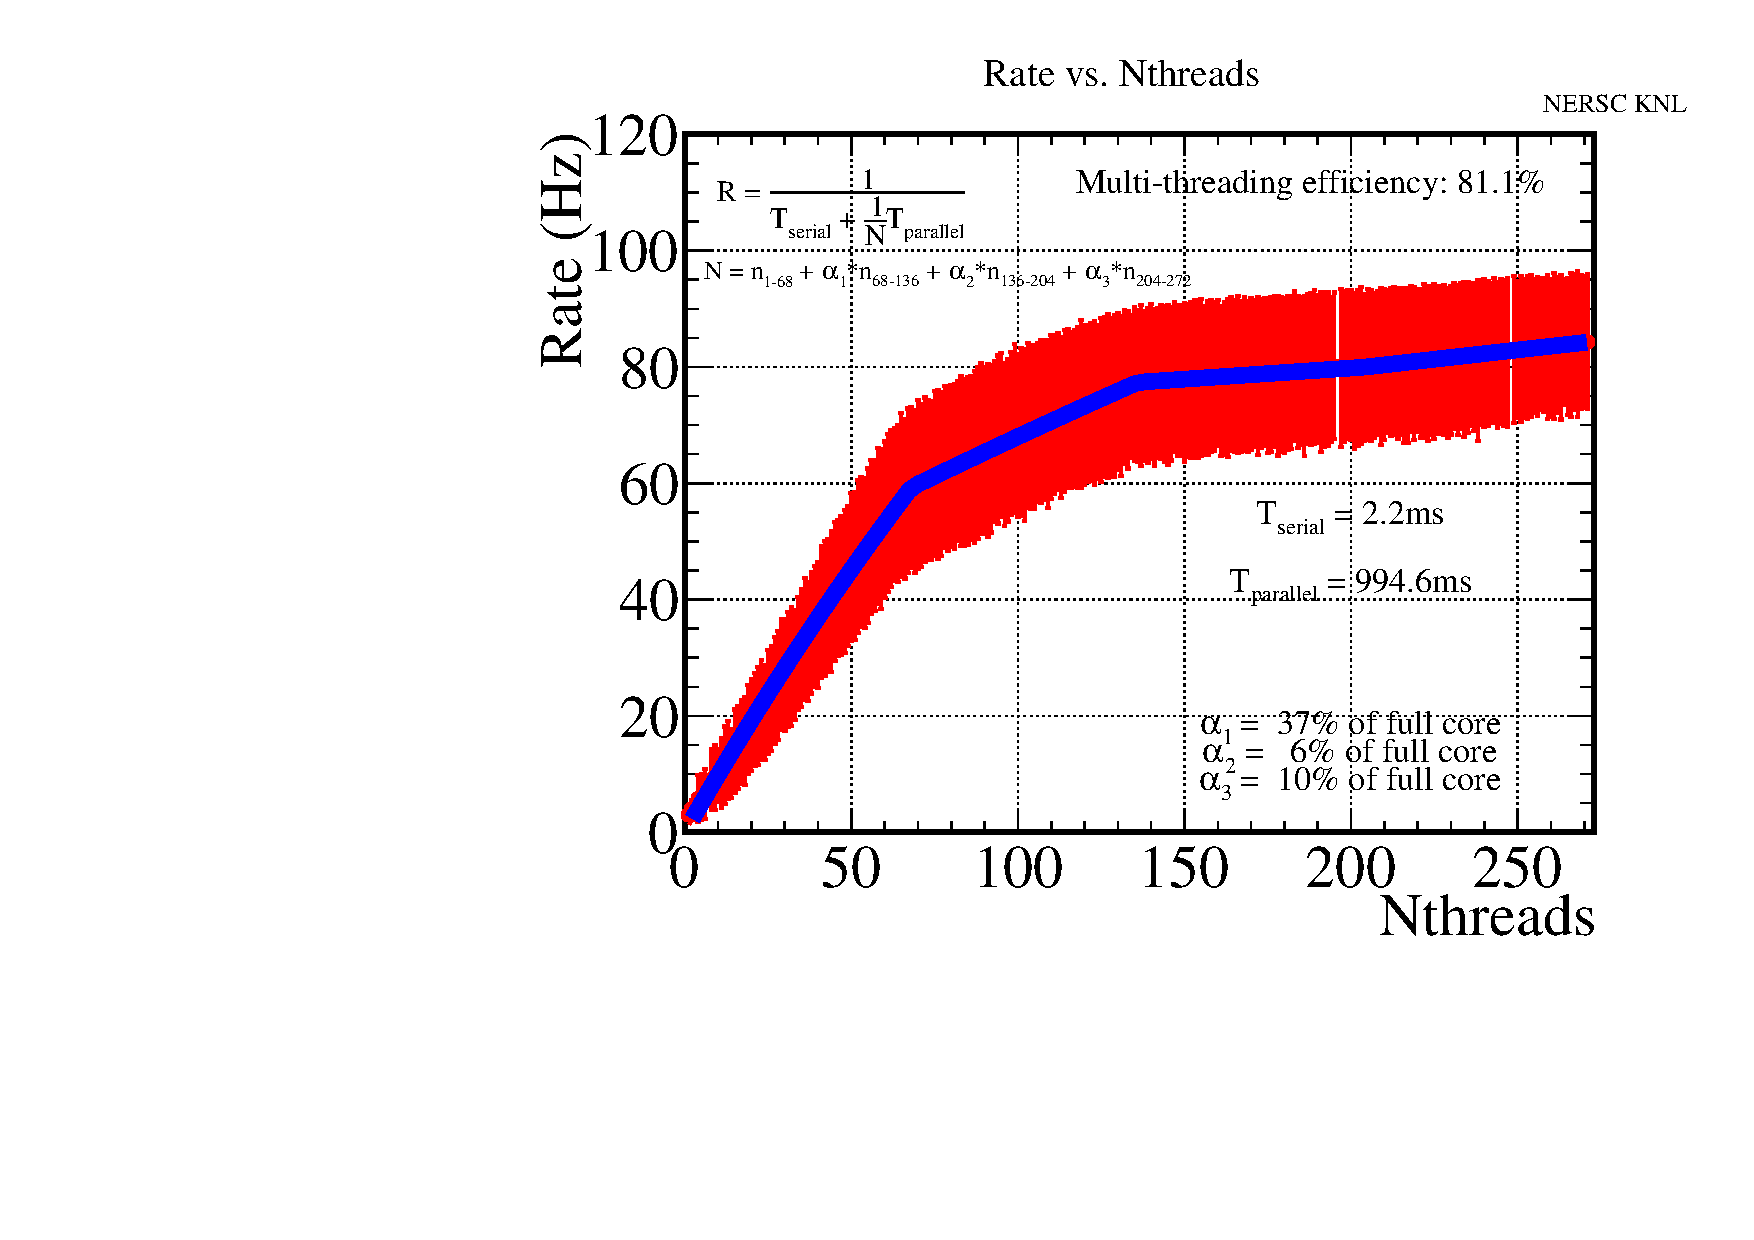
\includegraphics[width=0.49\textwidth]{figures/production_offsite_rate_vs_nthreads_NERSC.pdf}
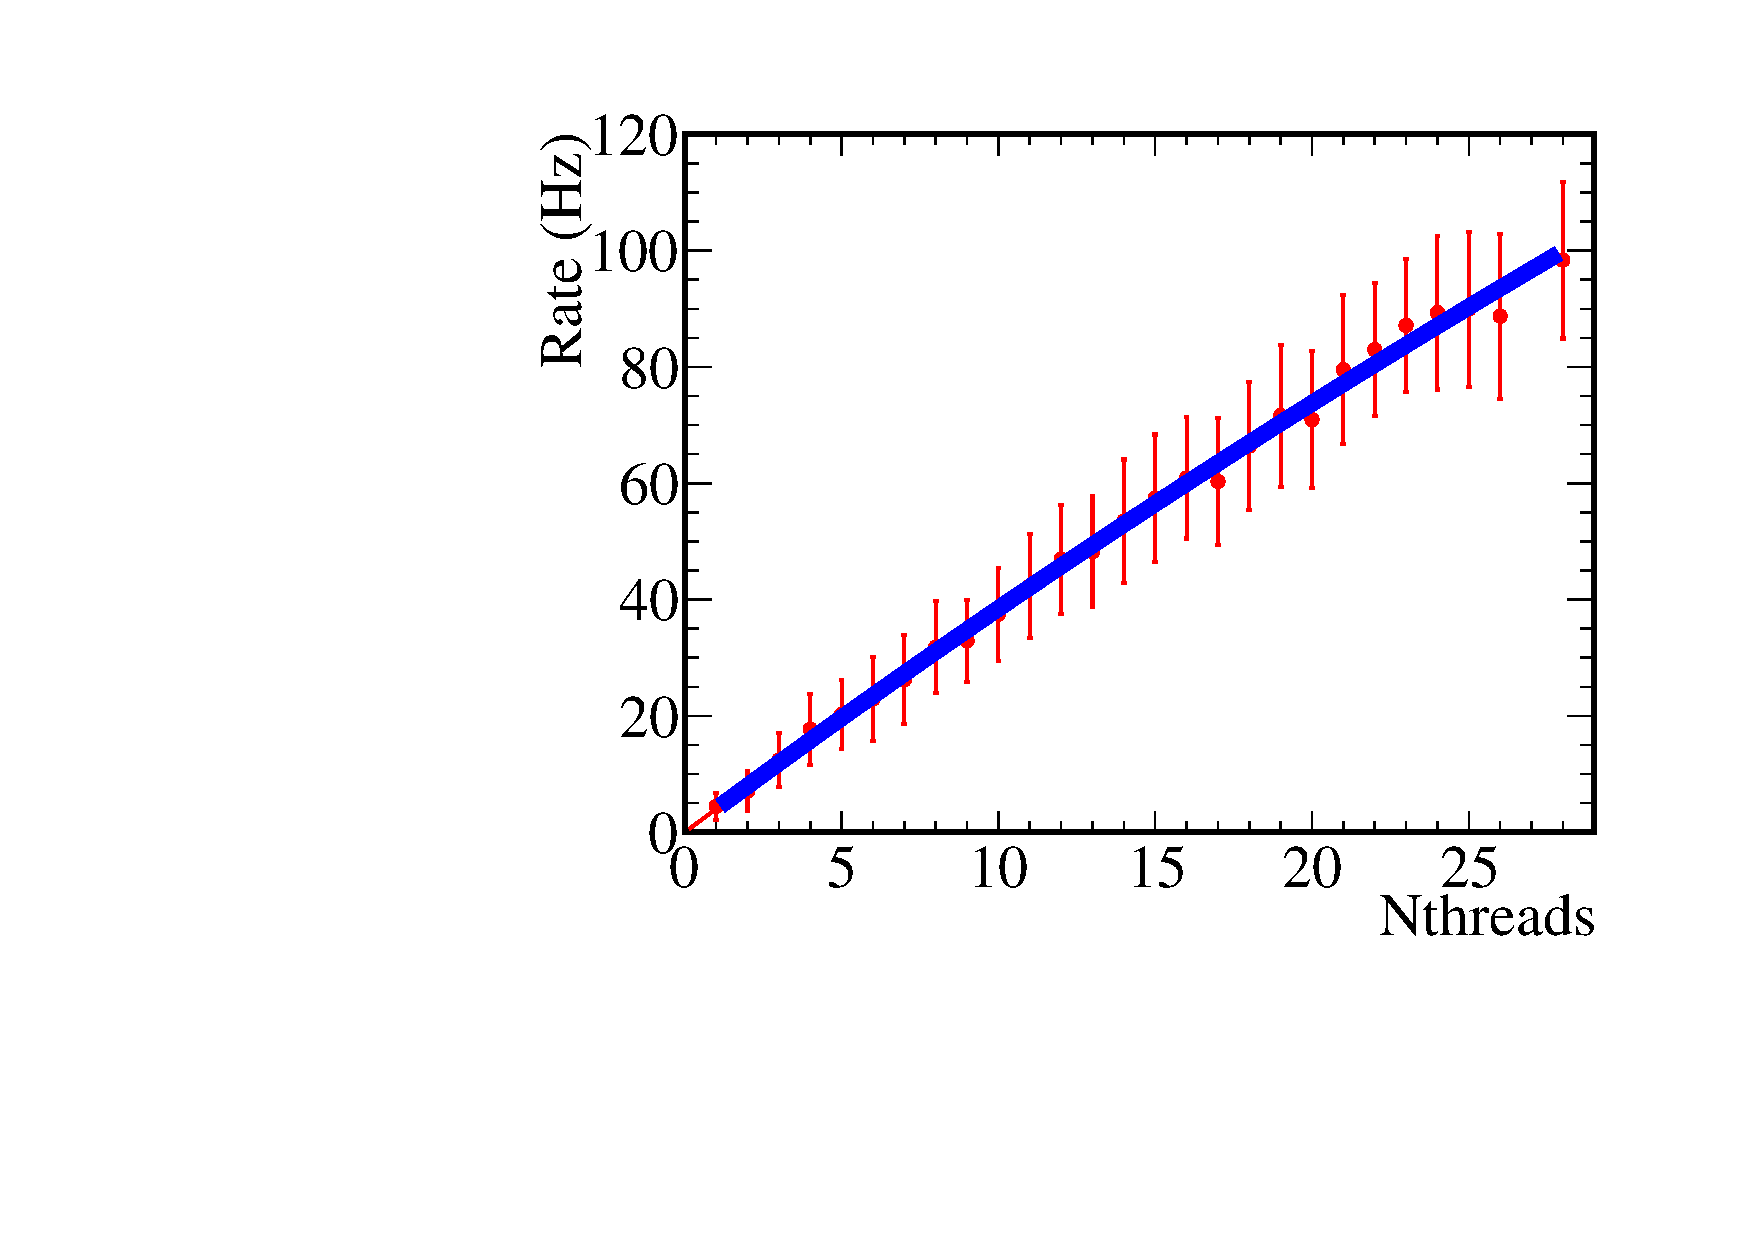
\includegraphics[width=0.49\textwidth]{figures/production_offsite_rate_vs_nthreads_PSC.pdf}
\caption[]{\label{fig:production_offsite_rate_vs_nthreads_NERSC}Event processing rate versus number of threads for reconstruction jobs on NERSC Cori II (left) and PSC Bridges (right). The structure in the NERSC plot is due to the KNL architecture, which had four hardware threads per core. For PSC Bridges, hyper-threading is disabled so no structure is observed.} 
\end{figure}

Container and distributed file system technologies were used for offsite processing. The software binaries as well as calibration constants, field maps etc. were distributed using the CERN-VM-file system (CVMFS). 
The binaries were all built at JLab using a CentOS7 system. A very lightweight Docker container was made based on CentOS7 that had only a minimal number of system RPMs\footnote{RedHat Package Management, https://access.redhat.com/documentation/en-us/red\_hat\_enterprise\_linux/5/html/deployment\_guide/ch-rpm} installed. All other software, including third-party packages such as ROOT, were distributed via CVMFS. This meant changes to the container itself were very rare (about once per year). The Docker container was pulled into NERSC's Shifter system without modification. The same container was used to create a Singularity container used at both PSC and on the Open Science Grid (OSG) for \GX~simulation jobs.


Raw data ware transferred from JLab to the remote sites using Globus\footnote{https://opensciencegrid.org/technology/policy/globus-toolkit.},  which uses GridFTP. The Globus tasks were submitted and managed by the SWIF2 workflow tool written by the JLab Scientific Computing group. SWIF2 was needed to manage the data retrieval from tape, for transfer to the remote site, for submission of remote jobs, and for transfer of processed data back to JLab. Disk space limitations at both JLab and the remote sites meant only a portion of the data set could be on disk at any one time. Thus, SWIF2 had to manage the jobs through all stages of data transfer and job submission.

%--------------------------------------------------------------------------
\subsection{Analysis \label{sec:recanalysis}}

The full reconstructed (REST) data is too large to be easily handled by individual analyzers. For that reason, a system was developed to analyze data at JLab and extract reaction-specific ROOT trees. This step is represented by the right-hand green box at the bottom of Fig.\,\ref{fig:production_overview}.

Users can specify individual reactions via a web interface.
%(see Fig.~\ref{fig:production_analysis}).
Periodically, the submitted reactions are downloaded into a configuration file, which steers the analysis launch. For each reaction, the \GX~analysis library inside the JANA framework creates possible particle combinations from the reconstructed charged tracks and showers saved in the REST format. Common selection criteria are applied for exclusivity and particle identification before performing a kinematic fit, using vertex and four-momentum constraints. Displaced vertices and inclusive reactions are also supported. Objects representing successful particle combinations (e.g. $\pi^0 \rightarrow \gamma\gamma$) and other objects are managed in memory pools, and can be reused by different channels to reduce the overall memory footprint of the process. With this scheme, up to one hundred different reactions can be combned into one launch over the reconstructed data.

If the kinematic fit converged for one combination of tracks and showers, the event was stored into a reaction-specific but generic ROOT tree, made accessible to the whole collaboration. The total size of these ROOT trees for the full data set strongly depend on the selected reaction, but are small enough to be copied to the user's home institution for a more detailed analysis.

%\begin{figure}[h!]\centering
%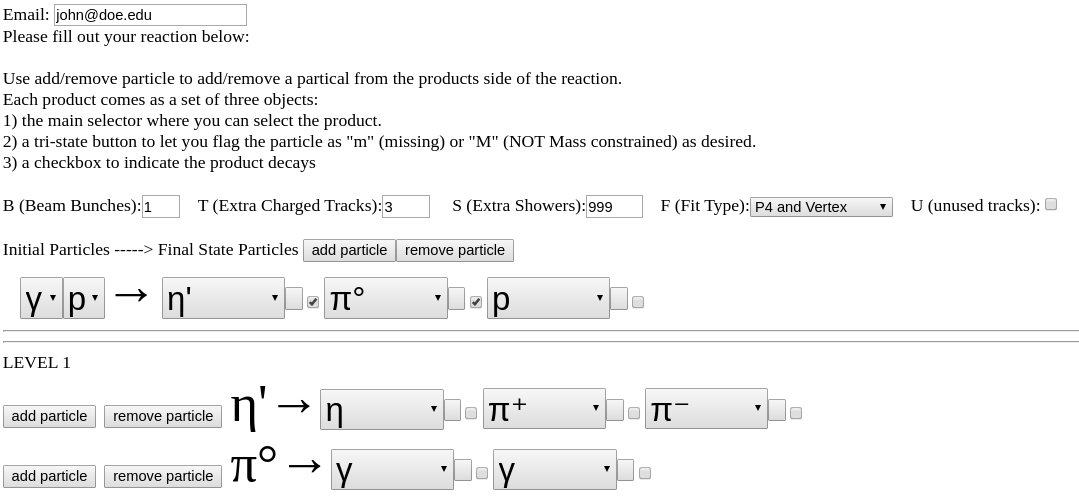
\includegraphics[width=\textwidth]{figures/analysis_submit_form.png}
%\caption[]{\label{fig:production_analysis}Analysis submission browser form.} 
%\end{figure}